\subsection{\label{sec:calib.dc}Drift Chamber Calibration and Resolution}

Tracking in the Drift Chamber of a \abbr{CLAS} Sector is performed using the six superlayers of the \abbr{DC}. A good measure of the the quality of tracking are the \abbr{DC} residuals for each superlayer. After a track is identified using the hit elements in the \abbr{DC} superlayer, It's \abbr{DC} residual is calculated using the TBLA bank as follows:

\begin{verbatim}
fabs(TBLA->tbla[i].fitdoca) - fabs(TBLA->tbla[i].calcdoca)
\end{verbatim}

\begin{v2}The Drift Chamber alignment was done by correcting the mean of the residuals and the results are shown in Fig.~\ref{fig:dc.align}.\end{v2}  The values of the \abbr{DC} residuals in the \abbr{CLAS} data are empirically found to be a good fit to a convolution of 2 Gaussians - a narrow Gaussian and a broad Gaussian. During \abbr{DC} calibrations efforts were made to minimize this residual to have maximum reconstruction efficiency. The mean and width of the residuals as a function of superlayer and run number are shown in Figs.~\ref{fig:calib.dc.residuals.mean} and \ref{fig:calib.dc.residuals.wid} respectively.

\begin{figure}\begin{center}
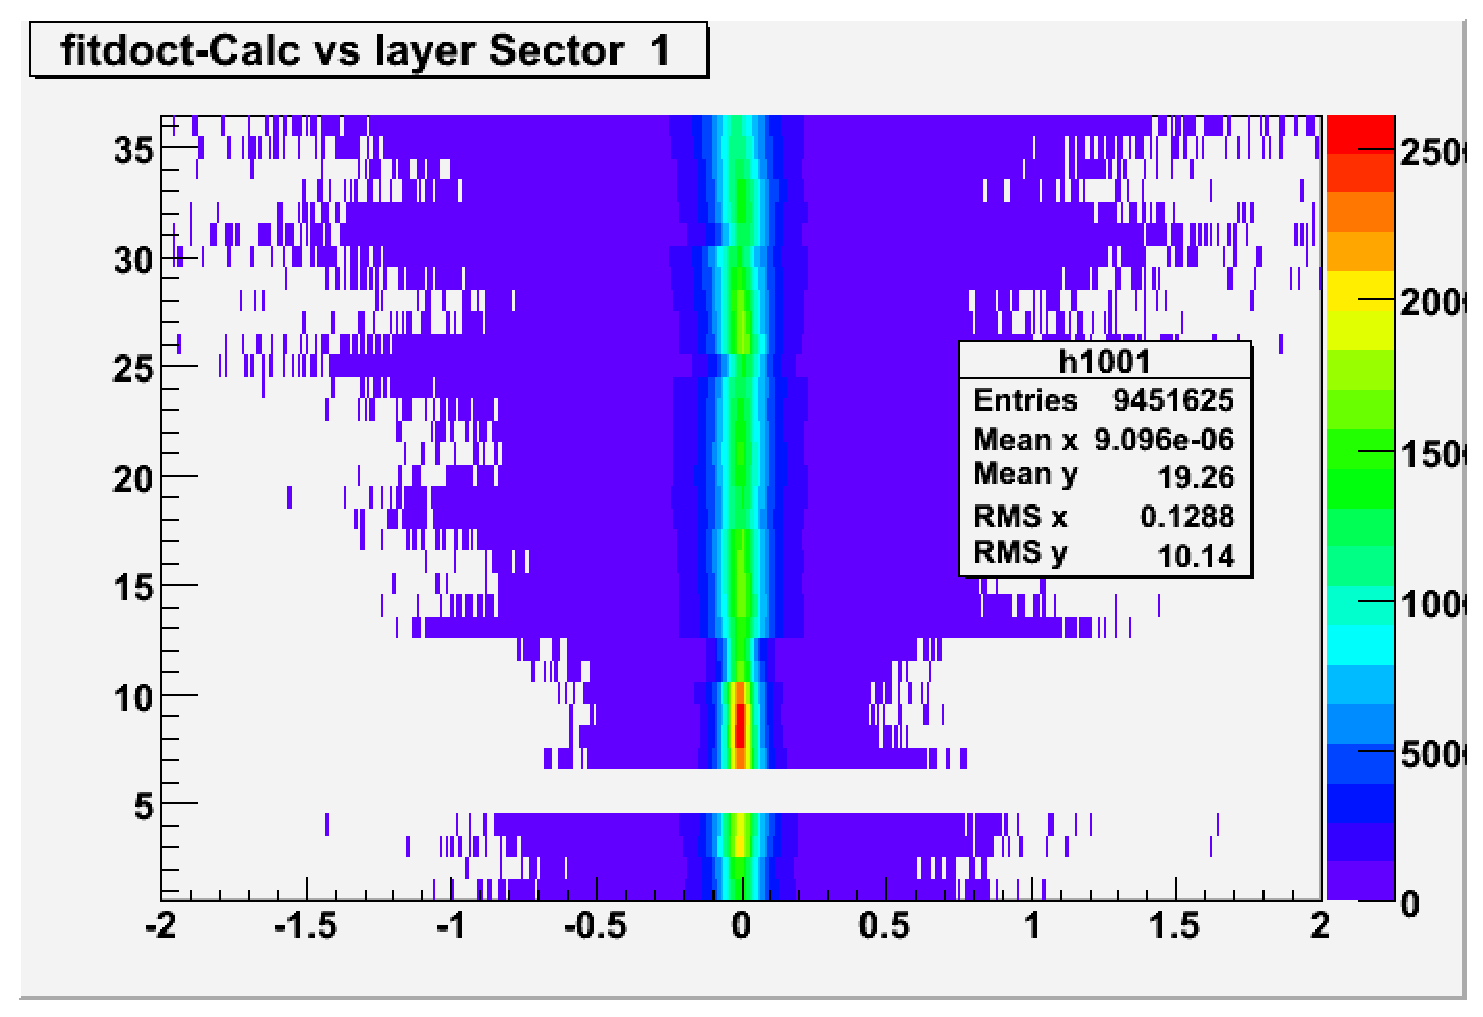
\includegraphics[width=0.6\textwidth]{figures/calib/dc/dc_align1.eps}
\caption[DC Alignment]{\label{fig:dc.align}Alignment of the Drift Chambers in sector 1. All other sectors show very similar results.}
\end{center}\end{figure}

\begin{figure}\begin{center}
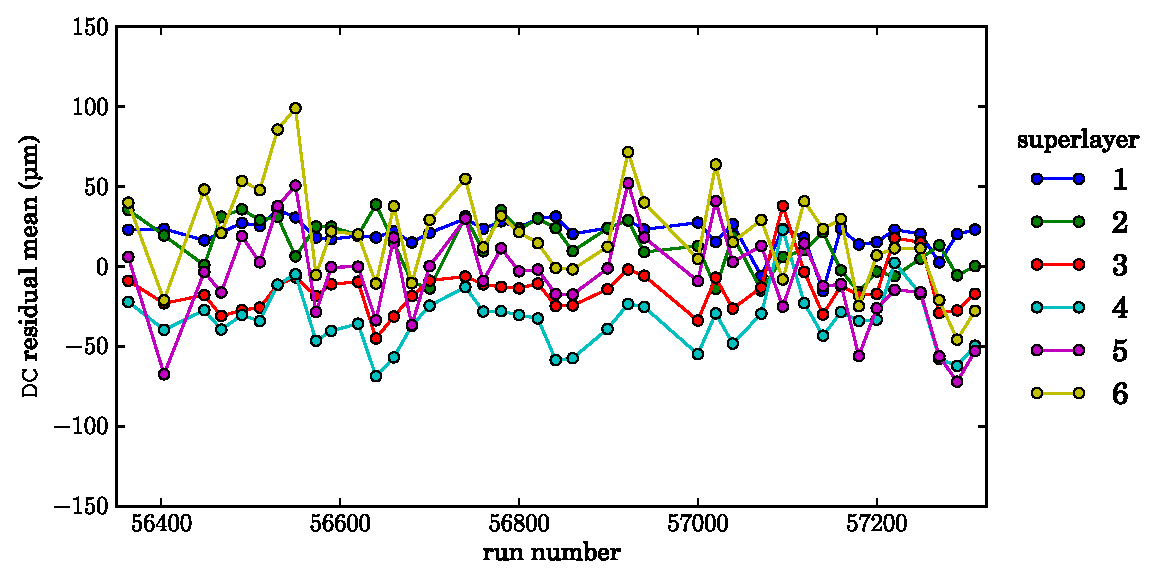
\includegraphics[width=0.6\textwidth]{figures/calib/dc/dc_resid_mean.eps}
\caption[DC Residuals (Mean)]{\label{fig:calib.dc.residuals.mean}Mean of residuals for the drift chambers by superlayer and by run.}
\end{center}\end{figure}

\begin{figure}\begin{center}
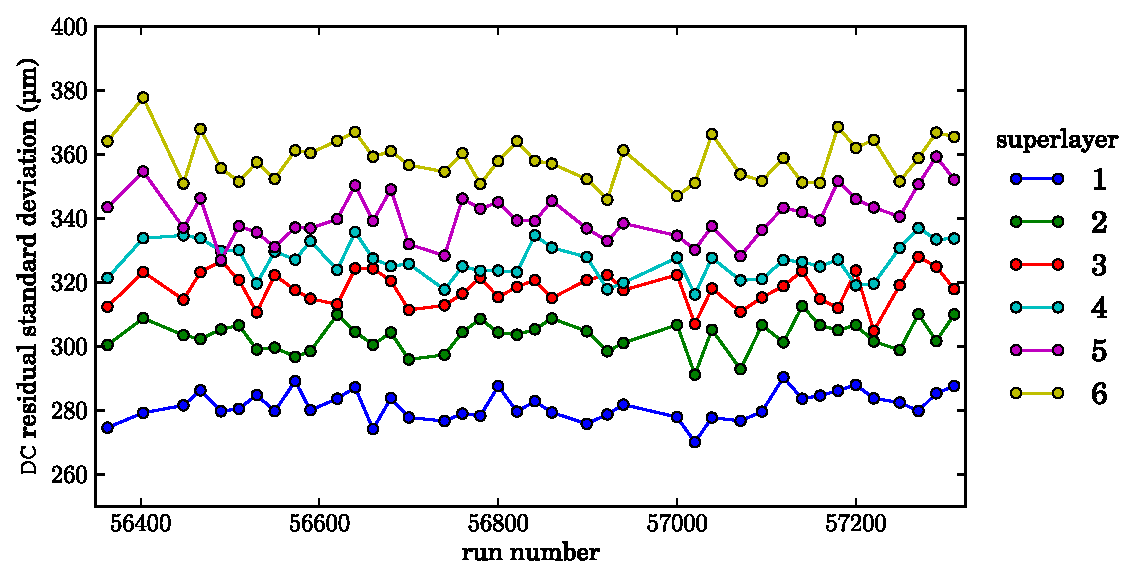
\includegraphics[width=0.6\textwidth]{figures/calib/dc/dc_resid_sigma.eps}
\caption[DC Residuals (Width)]{\label{fig:calib.dc.residuals.wid}Gaussian width of residuals for the drift chambers by superlayer and by run.}
\end{center}\end{figure}

\subsubsection{\label{sec:calib.dc.eff}Drift Chamber Wire Efficiency}

To generate the wire map for \desg{g12}, the utility \prog{pdu}, available in \abbr{SVN}, was used. Maurizio Ungaro made the wire-maps for \desg{g12} with the root files [\verb+A01+ and \verb+A02+] for each run. These output files are at \url{/home/mukesh/work/pdu_hbook} at \abbr{Jlab}. Root files needed are at \url{/home/mukesh/work/pdu_root}. The values were added to the \desg{g12} database. The results of the wire map are plotted in for each sector:

\begin{verbatim}
http://www.jlab.org/~ungaro/maureepage/proj/dceff/dc_periods/g12.html
\end{verbatim}

\FloatBarrier
